\documentclass[aspectratio=169]{beamer}
%\documentclass{beamer}
\usepackage{beamerthemeshadow}
\usecolortheme[RGB={21,96,189}]{structure}
\usepackage[english]{babel}
\usepackage{libertine}
\usepackage{tabularx,booktabs}
\newcolumntype{b}{>{\centering\arraybackslash}X}
\newcolumntype{s}{>{\centering\arraybackslash\hsize=.3\hsize}X}

\setbeamertemplate{headline}{}

%gets rid of bottom navigation bars
\setbeamertemplate{footline}[frame number]{}

%gets rid of bottom navigation symbols
\setbeamertemplate{navigation symbols}{}

%gets rid of footer
%will override 'frame number' instruction above
%comment out to revert to previous/default definitions
\setbeamertemplate{footline}{}

\title{\ldots} 
\author{\ldots}
\date{\ldots}
\institute{\large IIIA-CSIC}
\titlegraphic{\includegraphics[width=4cm]{logos/logoiiia-gran}}

\begin{document}

%\frame{\titlepage}

\newcommand{\inline}[1] { 
\mathord{\raisebox{-0.5ex}{\includegraphics[height=2.5ex]{img/#1}}} 
}

\frame{
\begin{block}{}
\centering
\vspace{20pt}
{\huge ONLINE LARGE-SCALE OPTIMISATION}
\vskip10pt
{\Large On-going research project @ IIIA-CSIC\\on \emph{ridesharing} using real-world data (NYC taxi dataset)}
\vskip15pt
\setlength{\fboxsep}{0pt}\fbox{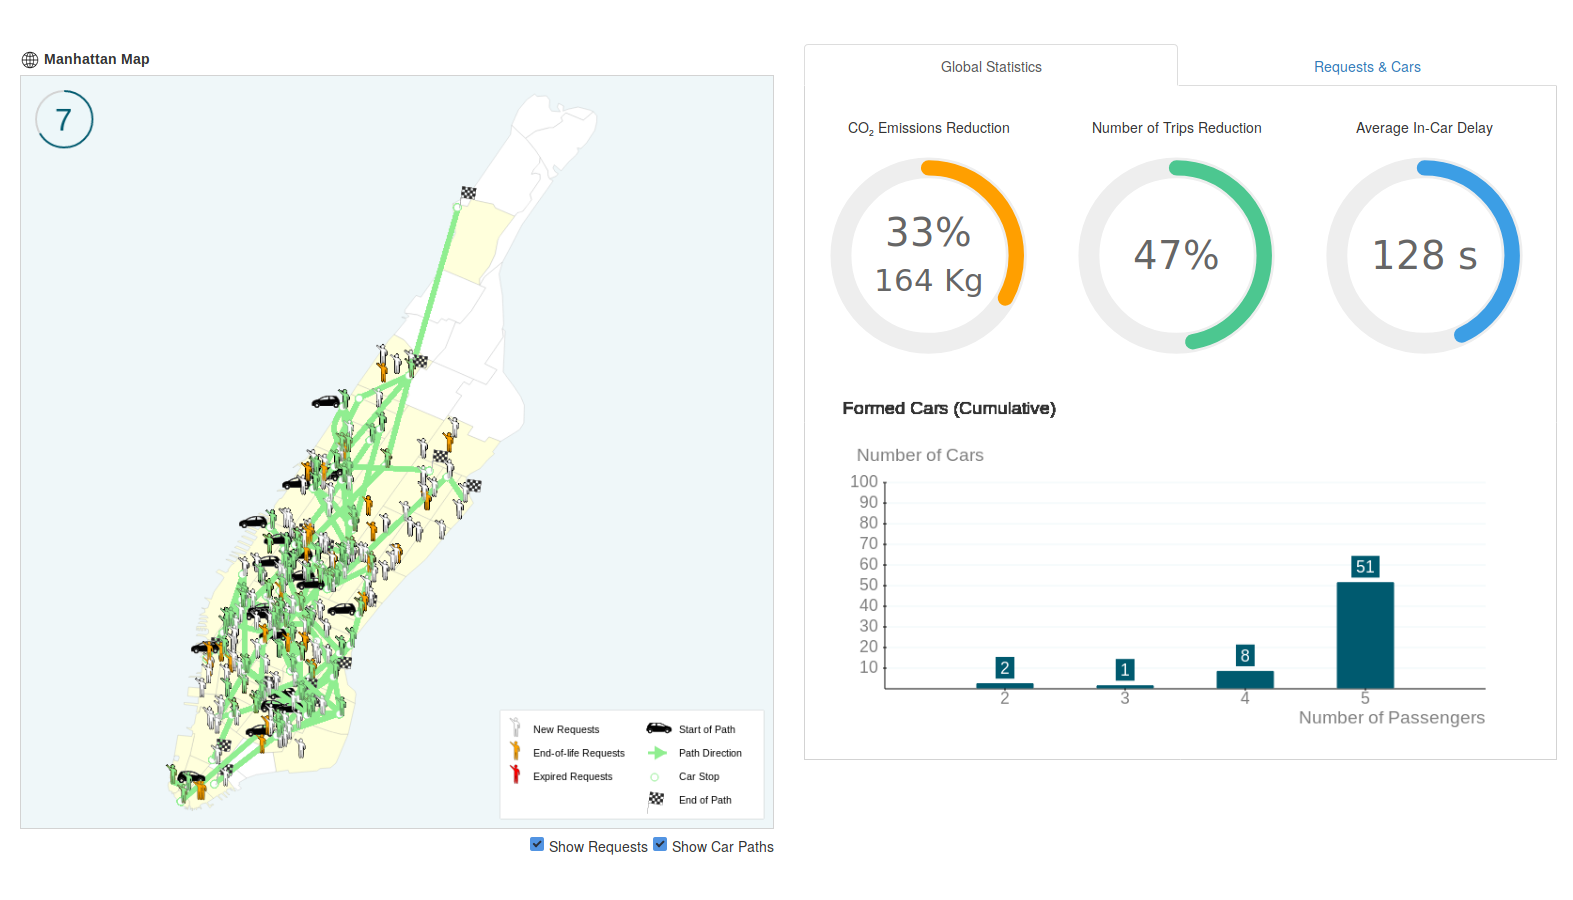
\includegraphics[width=0.4\linewidth]{img/demo.png}}
\vspace{20pt}
\end{block}
}

\frame{
\begin{block}{}
\centering
\vspace{20pt}
{\huge RESEARCH PROJECT}
\vskip10pt
{\Large Generation of \emph{good quality feasible solutions}\\when search space is too large to be fully explored}
\vspace{20pt}
\end{block}
}

\frame{
\begin{block}{}
\centering
\vspace{20pt}
{\huge HYPOTHESIS}
\vskip10pt
{\Large \emph{Generative Adversarial Networks} (GANs) can help us!}
\vskip15pt

\includegraphics[width=0.4\textwidth]{img/superman}
\vspace{20pt}
\end{block}
}

\frame{
\begin{block}{}
\centering
\vspace{20pt}
{\huge WHAT IS A GAN?}
\vskip10pt
{\Large Deep learning model able to learn how to \emph{generate}\\new samples from a dataset of examples}
\vskip15pt

\includegraphics[width=0.76275\textwidth]{img/gan}
\vspace{20pt}
\end{block}
}

\frame{
\begin{block}{}
\centering
\vspace{20pt}
{\huge THE PROJECT}
\vskip10pt
{\Large 
\begin{enumerate}
\item Learn how to use PyTorch
\item Learn how to use GANs
\item Apply GANs to toy problem (small dataset, existing code)
\item Apply GANs to ridesharing using NYC dataset (research part)
\item Write report/research article
\end{enumerate}
}
\vspace{20pt}
\end{block}
}

\end{document}
